% Joaquin Matres
%%%%%%%%%%%%%%%%%%%%%%% preamble %%%%%%%%%%%%%%%%%%%%%%%%%%%
\documentclass[10pt,letterpaper]{article}
\usepackage{opex3}
\usepackage{amsmath}

\usepackage{color}
\newcommand{\comment}[1]{\textcolor{red}{#1}}
% \usepackage{ae} %%for Computer Modern fonts

%%%%%%%%%%%%%%%%%%%%%%% begin %%%%%%%%%%%%%%%%%%%%%%%%%%%%%%
\begin{document}

%%%%%%%%%%%%%%%%%% title page information %%%%%%%%%%%%%%%%%%
\title{Low TPA and free-carrier effects in silicon nanocrystal-based horizontal slot waveguides}
%\title{Low carriers silicon nanocrystal-based horizontal slot waveguide}
\author{J. Matres$^{*,1}$, C. Lacava$^2$, G. C. Ballesteros$^1$, P. Minzioni$^2$, I. Cristiani$^2$, J.~M.~F\'ed\'eli$^3$, J. Mart\'i$^1$ and C. J. Oton$^1$} 
\address{$^1$ Nanophotonics Technology Center, \\ Universidad Polit\'ecnica de Valencia, Camino de Vera s/n, 46022, Valencia, Spain\\
$^2$Dipartimento di Ingegneria Industriale e dell'Informazione, Universita di Pavia, Via Ferrata 1, 27100, Pavia, Italy\\
$^3$CEA LETI, Minatec Campus, Grenoble 38054, France}
\email{$^*$joamatab@ntc.upv.es}


%%%%%%%%%%%%%%%%%%% abstract and OCIS codes %%%%%%%%%%%%%%%%
%% [use \begin{abstract*}...\end{abstract*} if exempt from copyright]

\begin{abstract}
We present the characterization of the ultrafast nonlinear dynamics of a CMOS-compatible horizontal-slot waveguide with silicon nanocrystals. Results are compared to strip silicon waveguides, and modeled with nonlinear split-step calculations. The extracted parameters show that the slot waveguide has weaker carrier effects and better nonlinear figure-of-merit than the strip waveguides. 
\end{abstract}

\ocis{(190.0190) Nonlinear optics; (130.0130) Integrated optics; (320.0320) Ultrafast optics; (160.4330) Nonlinear optical materials.}

%(220.0220) Optical design and fabrication; (230.5750) Resonators; (230.3990) Microstructure devices; (250.5300) Photonic Integrated Circuits.}

%%%%%%%%%%%%%%%%%%%%%%% References %%%%%%%%%%%%%%%%%%%%%%%%%
\bibliographystyle{osajnl}

\begin{thebibliography}{10}
\newcommand{\enquote}[1]{``#1''}

\bibitem{Almeida2004a}
V.~Almeida, C.~Barrios, and R.~Panepucci, \enquote{{All-optical control of
  light on a silicon chip},} Nature \textbf{431}, 1081--1084 (2004).

\bibitem{Lee2009}
B.~Lee and A.~Biberman, \enquote{{Demonstration of broadband wavelength
  conversion at 40 Gb/s in silicon waveguides},} Photonics \textbf{21},
  182--184 (2009).

\bibitem{Koos2009}
C.~Koos, P.~Vorreau, T.~Vallaitis, P.~Dumon, W.~Bogaerts, R.~Baets,
  B.~Esembeson, I.~Biaggio, T.~Michinobu, F.~Diederich, W.~Freude, and
  J.~Leuthold, \enquote{{All-optical high-speed signal processing with silicon
  � organic hybrid slot waveguides},} Nature Photonics \textbf{3}, 1--4
  (2009).

\bibitem{Sanchis2007}
P.~Sanchis, J.~Blasco, A.~Martinez, and J.~Marti, \enquote{{Design of
  Silicon-Based Slot Waveguide Configurations for Optimum Nonlinear
  Performance},}  (2007).

\bibitem{Spano2009}
R.~Spano, N.~Daldosso, M.~Cazzanelli, L.~Ferraioli, L.~Tartara, J.~Yu,
  V.~Degiorgio, E.~Giordana, J.~M. Fedeli, and L.~Pavesi, \enquote{{Bound
  electronic and free carrier nonlinearities in Silicon nanocrystals at
  1550nm.}} Optics Express \textbf{17}, 3941--3950 (2009).

\bibitem{Martinez2010a}
A.~Mart\'{\i}nez, J.~Blasco, P.~Sanchis, J.~V. Gal\'{a}n,
  J.~Garc\'{\i}a-Rup\'{e}rez, E.~Jordana, P.~Gautier, Y.~Lebour,
  S.~Hern\'{a}ndez, R.~Guider, N.~Daldosso, B.~Garrido, J.~M. Fedeli,
  L.~Pavesi, J.~Mart\'{\i}, and R.~Spano, \enquote{{Ultrafast all-optical
  switching in a silicon-nanocrystal-based silicon slot waveguide at telecom
  wavelengths.}} Nano letters \textbf{10}, 1506--11 (2010).

\bibitem{Otona}
C.~J. Oton, J.~Matres, P.~Sanchis, J.~P. Colonna, C.~Ratin, and J.~M. Fedeli,
  \enquote{{Ultrafast all-optical logic gates with silicon nanocrystal-based
  slot waveguides},} IEEE Group IV Photonics pp. 171--173 (2010).

\bibitem{Trita2011}
A.~Trita, C.~Lacava, P.~Minzioni, J.-P. Colonna, P.~Gautier, J.-M. Fedeli, and
  I.~Cristiani, \enquote{{Ultra-high four wave mixing efficiency in slot
  waveguides with silicon nanocrystals},} Applied Physics Letters \textbf{99},
  191105 (2011).

\bibitem{Vallaitis2008}
T.~Vallaitis, C.~Koos, R.~Bonk, W.~Freude, M.~Laemmlin, C.~Meuer, D.~Bimberg,
  and J.~Leuthold, \enquote{{Slow and fast dynamics of gain and phase in a
  quantum dot semiconductor optical amplifier.}} Optics express \textbf{16},
  170--8 (2008).

\bibitem{Vallaitis2009}
T.~Vallaitis, S.~Bogatscher, L.~Alloatti, P.~Dumon, R.~Baets, M.~L. Scimeca,
  I.~Biaggio, F.~Diederich, C.~Koos, W.~Freude, and J.~Leuthold,
  \enquote{{Optical properties of highly nonlinear silicon-organic hybrid (SOH)
  waveguide geometries.}} Optics express \textbf{17}, 17357--68 (2009).

\bibitem{Agrawal2001a}
G.~P. Agrawal, \emph{{Nonlinear Fiber Optics}}, vol.~15 of \emph{Optics and
  Photonics} (Academic Press, 2001).

\bibitem{Lin2007}
Q.~Lin, O.~J. Painter, and G.~P. Agrawal, \enquote{{Nonlinear optical phenomena
  in silicon waveguides: modeling and applications.}} Optics express
  \textbf{15}, 16604--44 (2007).

\bibitem{Mas2012}
S.~Mas, J.~Matres, J.~Mart\'{\i}, and C.~J. Oton, \enquote{{Accurate Chromatic
  Dispersion Characterization of Photonic Integrated Circuits},} IEEE Photonics
  Journal \textbf{4} (3) 825--831 (2012).
\end{thebibliography}



\section{Introduction}
Nonlinear silicon-based photonic devices can introduce key functionalities for on-chip optical signal processing and routing. In the last years, many different nonlinear silicon devices have been reported, such as all-optical modulators~\cite{Almeida2004a}, wavelength converters~\cite{Lee2009}, demultiplexers~\cite{Koos2009}, etc. These nonlinear devices can be based either on free carriers or on the bound-electron Kerr coefficient. In pure silicon waveguides, the Kerr effect is usually hindered by more intense and longer-lasting free-carrier dispersion (FCD). However, it is often desirable to exploit the Kerr effect, as its temporal response is instantaneous (thus allowing high-speed operation) and it enables parametric conversion and amplification. In order to increase the Kerr coefficient and reduce carrier effects in silicon waveguides, a slot-type geometry was proposed~\cite{Sanchis2007}, where a thin layer of a low-index material material with high nonlinear coefficient is sandwiched between two 
silicon channels. A vertical slot geometry was also demonstrated to allow the introduction of an organic polymer, and this device showed optical 160~Gb/s demultiplexing capabilities~\cite{Koos2009}; however, these materials involve non-CMOS processes and impose strict temperature limitations. On the other hand, silicon-nanocrystal-based horizontal slot waveguides only require CMOS processes, and have recently demonstrated ultrafast all-optical modulation capabilities and good nonlinear properties~\cite{Spano2009, Martinez2010a, Otona, Trita2011}. In this paper, we study the nonlinear ultrafast dynamics of this type of waveguide, where we show that the effect of carriers is greatly reduced as compared to silicon channel waveguides. We also report quantitative measurements of nonlinear absorption of these waveguides. Finally we show simulation results which fit the experimental results and provide estimations of the nonlinear parameters and figures of merit of the waveguides.


\section{Fabrication}
Slot samples were fabricated starting from silicon--on--insulator (SOI) wafers with 220~nm Si thickness. On top of the Si layer, a 100~nm--thick layer of silicon--rich silica ($ \mathrm{SiO_x} $) was grown by plasma-enhanced chemical vapor deposition (PECVD), and annealed at 1000~\textcelsius ~in $ \mathrm{N}_2 $ ambient for 210~s. The nominal amount of silicon excess was 16\% and Silicon-nanocrystals had an average size of 4~nm. On top of that layer, a 240~nm-thick layer of amorphous Si was grown by PECVD to form the top half of the waveguide. Waveguides were patterned with deep-UV lithography and etched down to the buried oxide to form channels as the ones reported in~\cite{Martinez2010a, Trita2011}. The whole layout was covered with silica after the etching process as shown in Fig.~\ref{fig:semSlot}. On the other hand, two Si strip waveguides were fabricated for comparison, always starting  from SOI wafers patterned with deep-UV lithography. Their dimensions were $445\times220$~nm for transverse-electric (
TE) polarization and $485\times220$~nm for transverse-magnetic 
(TM) polarization, both with a length of 25~mm. The slot waveguide, where the TM-polarized mode was excited to exploit the E-field magnification effect in the slot region, was 7~mm long.


\begin{figure}[htb]
\centering
\includegraphics[width=0.42\textwidth]{slot2d}%0.6
\caption{Silicon-nanocrystals (Si-nc) slot waveguide schema. Top made of amorphous silicon (a-Si) and bottom of crystalline silicon (c-Si)}
\label{fig:semSlot}
\end{figure}


\section{Nonlinear loss measurements: Im$ (\gamma) $}
\label{sec:imGamma}
First, we characterized the nonlinear loss in all the samples under test.  Two-photon absorption (TPA) is a well-known process in silicon waveguides, and can be considered as the imaginary part of the gamma coefficient using the differential equation:

\begin{equation}
\frac{dP}{dz} = -\alpha P(z) - 2|Im(\gamma)| P(z)^2 
\label{eq:differentialTPA}
\end{equation}

where $P$ is the signal power through the waveguide, $\alpha$ is the linear loss of the waveguide, and Im$(\gamma)$ is the imaginary part of the $\gamma$ coefficient (we use the absolute value because Im$(\gamma)$ is negative, but we want to stress its loss character in the equation with a negative sign). 
The solution of the differential equation shown in Eq.~\ref{eq:differentialTPA} after a distance $L$ is given by:

                                                                \begin{equation}
                                                                         P(L) = \frac{e^{-\alpha_0 L}}{1+2|Im(\gamma)| L_{eff} P_0} P_0
                                                                \end{equation}

where $P_0$ is the input power in the waveguide. Therefore the impact of nonlinear losses on the overall transmission ($T_{NL}$) can be calculated as the ratio between the transmission at high power ($T_{HP} = P(L)/P_0 $) and the transmission at low power ($T_{LP} = e^{-\alpha_0 L} $). In particular the inverse of $T_{NL}$ turns out to be a linear function of $P_0$:

                                                                \begin{equation}
                                                                         T_{NL}^{-1} = \frac{T_{LP}}{T_{HP}} = 1+2|Im(\gamma)| L_{eff} P_0
                                                                        \label{eq:transmissionLinear}
                                                                \end{equation}

As a consequence, if we plot this ratio as a function of $P_0$, the slope of the curve can give us the two-photon absorption coefficient of our waveguide as in~\cite{Vallaitis2009}.
However, this equation is only valid for instantaneous transmission values. When a pulsed signal $P_0(t)$ is launched into the waveguide, the measured transmission is time-averaged, and the equivalent $T_{NL}^{-1}$ can be expressed as:

                                                                \begin{equation}
                                                                        \tilde{T}_{NL}^{-1} = \frac{\tilde{T}_{LP}}{\tilde{T}_{HP}} = \frac{\int P_0(t)dt}{\int \frac{P_0(t)}{1+2|Im(\gamma)| L_{eff} P_0(t)} dt}
                                                                        \label{eq:transmissionIntegral}
                                                                \end{equation}

If the pulsed signal has a rectangular shape, one can use Eq.~\ref{eq:transmissionLinear}, but if the shape is different, the integral in Eq.~\ref{eq:transmissionIntegral} must be solved, as the result differs significantly. The reason for this variation is the fact that the flanks of the pulse are not affected as hardly by TPA as the peak. Therefore, the overall energy transmission is higher than for the case of cw excitation. For the particular case of a $sech^2$ shape, which corresponds to the output of our laser, emitting 1-ps pulses with a repetition rate of 20~MHz and a central wavelength of 1539~ nm, the result of  Eq.~\ref{eq:transmissionIntegral} is given by:


                                                                \begin{equation}
                                                                        \tilde{T}_{NL}^{-1}  = \frac{\tilde{T}_{LP}}{\tilde{T}_{HP}} \bigg|_{sech^2~shape}  = \frac{\sqrt{\delta({\delta + 1})}}{\ln(\sqrt{\delta}+\sqrt{\delta+1})} ~~\mathrm{where}~~  \delta = 2|Im(\gamma)| L_{eff} P_{0 peak}
                                                                        \label{eq:transmissionHypSecant}
                                                                \end{equation}


We measured the $T_{LP}$ and $T_{HP}$ parameters by putting a variable attenuator at the laser output and using a power-meter. The experimental results are shown in Fig.~2, together with the fitting curves obtained using Eq.~\ref{eq:transmissionHypSecant} in order to extract the Im$(\gamma)$ parameter shown in Table \ref{tab:results}. 
%%%PAVIA%%%%%%%%%We have to comment a bit the results about Im Gamma so we can propose to write down this part:
It is worth noting that the Im$(\gamma )$ of slot waveguides is much lower than that of TE strip-waveguide. This can be easily explained considering that in the slot structure the main part of the optical field is confined within the region containing silicon oxide doped with silicon nanocrystals, which have a band-gap higher than that of Silicon. The low value of Im$(\gamma)$ measured in TM strip-waveguide is due to the fact that  the mode largely extends in the $\mathrm{SiO_2}$ cladding. 



\begin{figure}[htb]
    \centering
    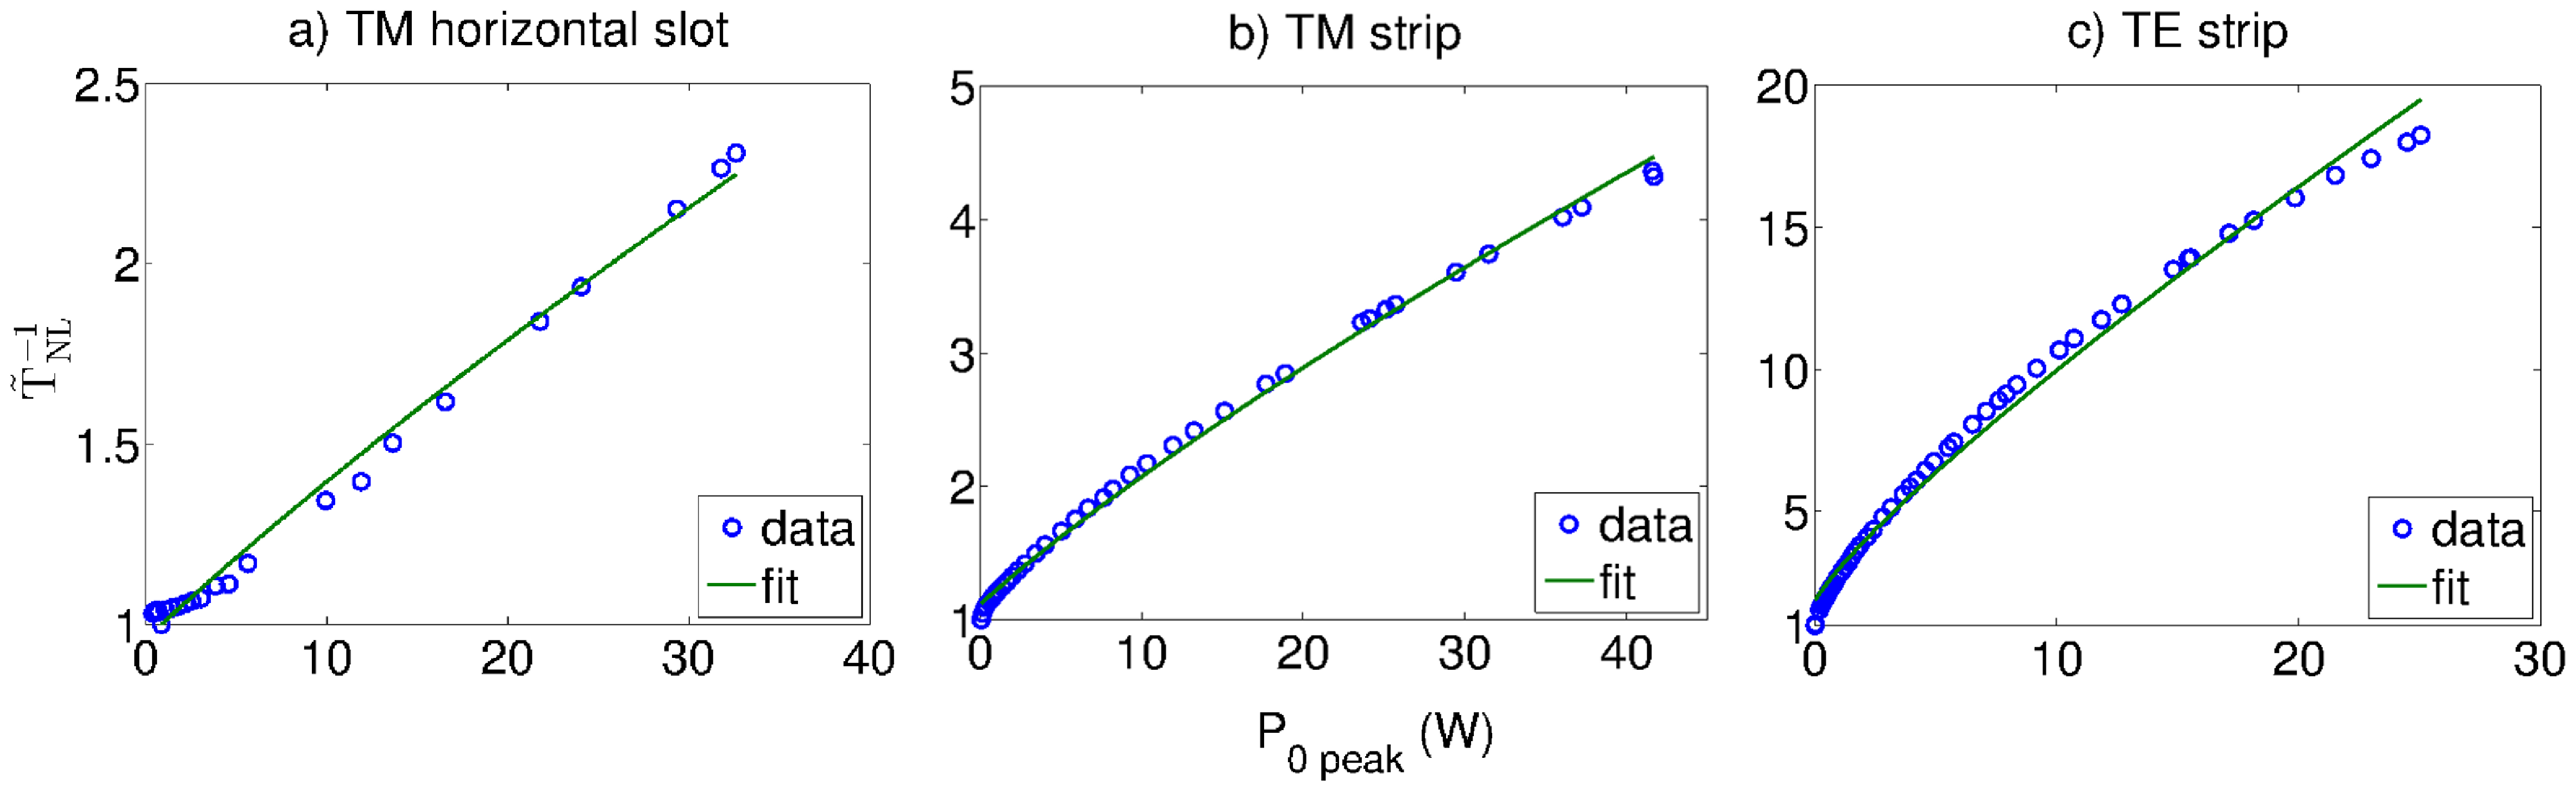
\includegraphics[width=1.0\textwidth]{imGamma_slot_TM_TE_v6}
     \caption{Transmission versus waveguide peak power (note the difference in the y-scale among the three plots). Solid line shows the fit for $ sech^2 $ pulses using Eq.~\ref{eq:transmissionHypSecant}.}
    \label{fig:imGammaSamples}
\end{figure}




                               % \begin{figure}[htb]
                                %   \centering
                                 %  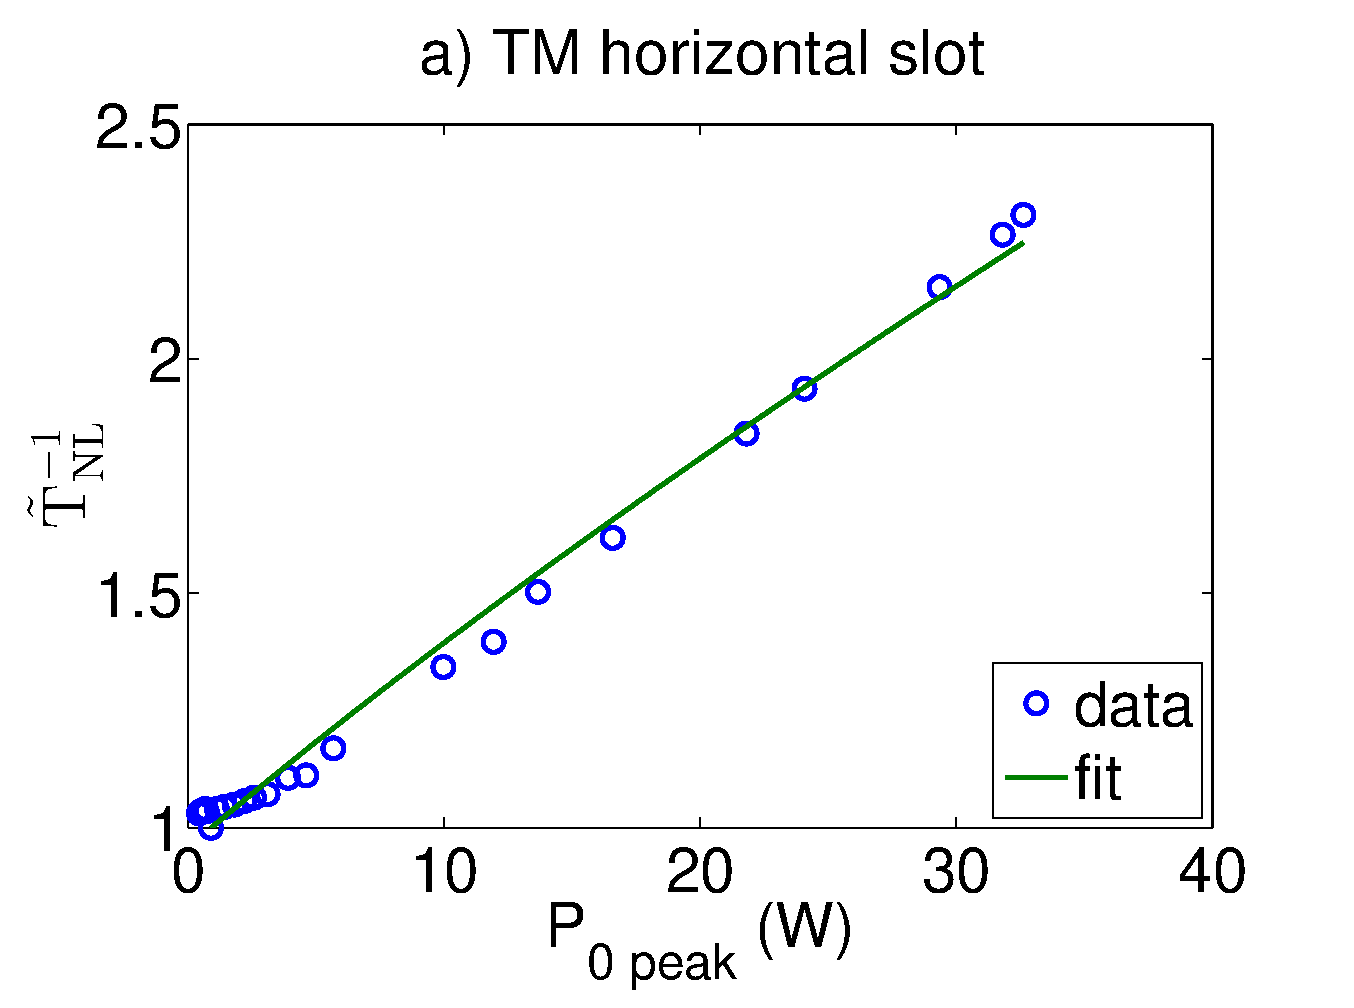
\includegraphics[width=0.32\textwidth]{imGamma_slot}
                                  % 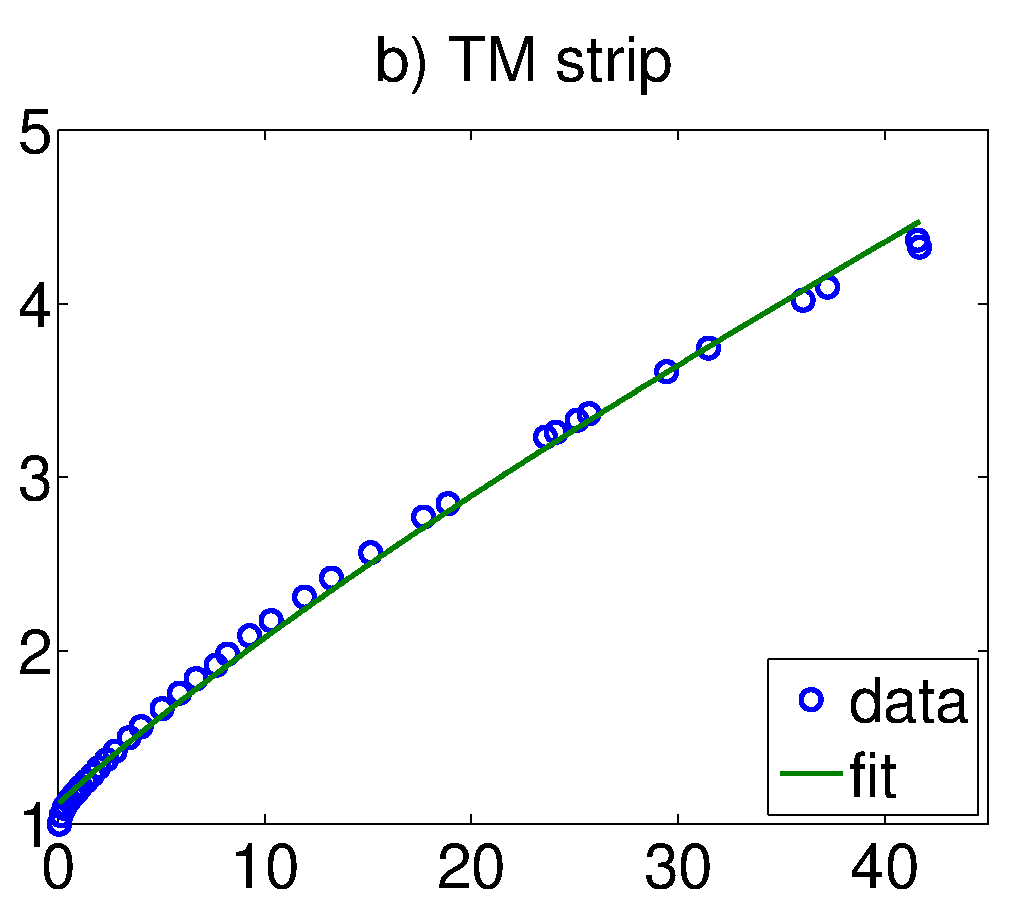
\includegraphics[width=0.32\textwidth]{imGammaTM}   
                                   %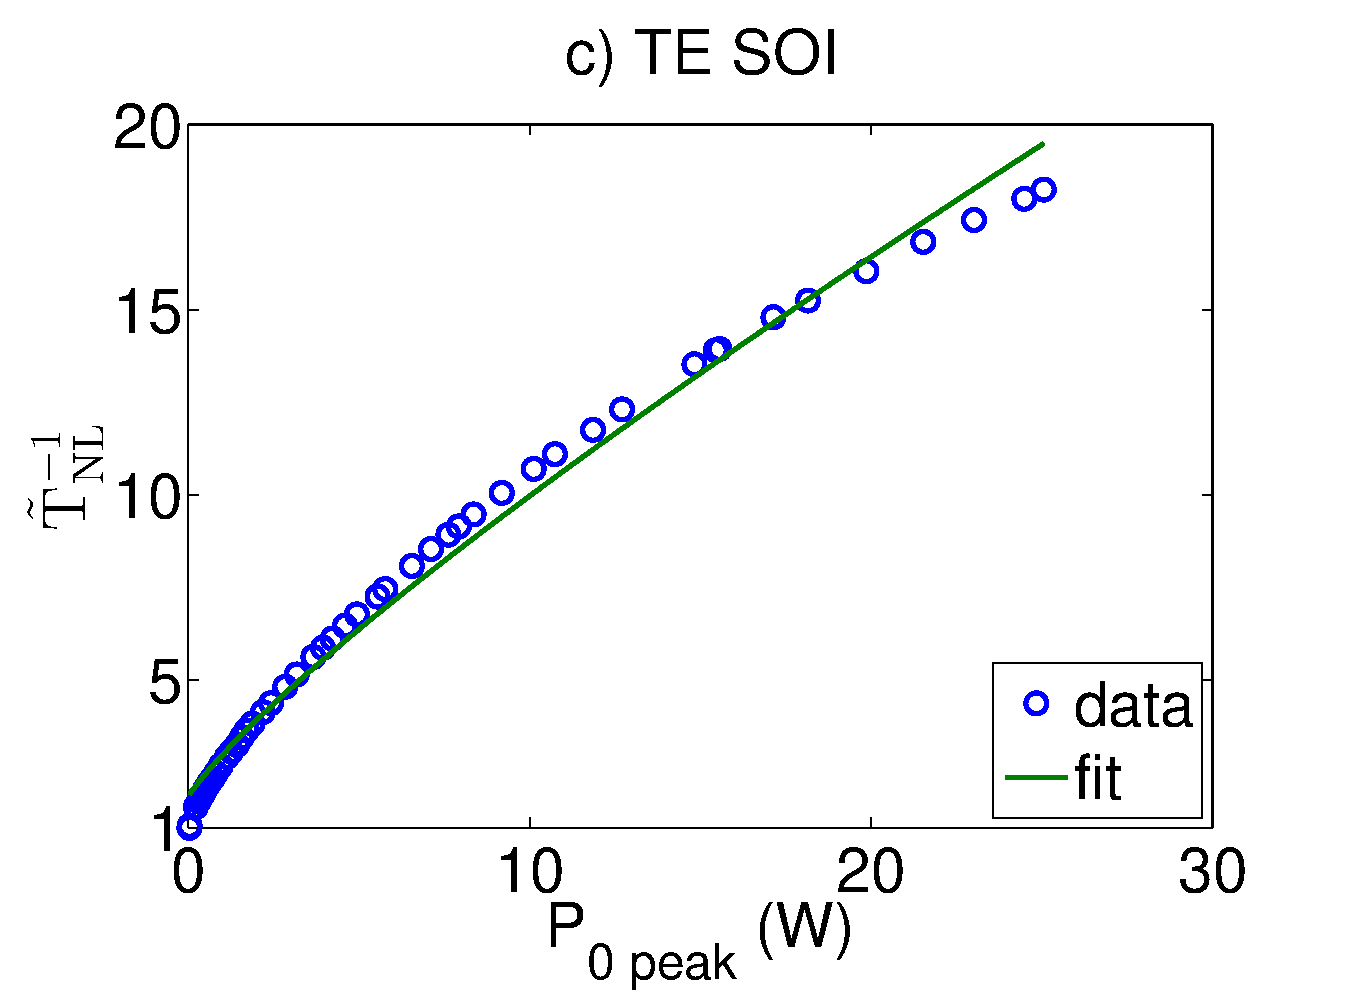
\includegraphics[width=0.32\textwidth]{imGammaTE}
                                   %\caption{Transmission versus waveguide peak power (note the difference in the y-scale among the three plots). Solid line shows the fit for $ sech^2 $ pulses using Eq.~\ref{eq:transmissionHypSecant}. LEGEND ON THE LEFT DOESN'T HAVE SYMBOLS. Y-LABEL SHOULD BE $\tilde{T}^{-1}$}
                                   %\label{fig:imGammaSamples}
                                %\end{figure}

\section{Time-resolved measurements}
Time resolved measurements were performed in order to distinguish Kerr and TPA from carrier effects, using the technique described in \cite{Vallaitis2008}. The set-up is shown in Fig.~3. We split the 1~ps pulse into three pulses: the most intense acts as a pump, while the two weaker pulses (reference and probe) are frequency shifted by two acousto-optic modulators (respectively by 80~MHz and 80.04~MHz ) and recombined with a fixed probe-to-reference delay of 10~ns. All the pulses are then coupled inside the waveguide under test and the time-delay between probe pulse and pump pulse is changed by means of a variable delay line. At the output, the probe and reference pulses are re-synchronized by a 10~ns delay-line and their beating signal is recovered by a lock-in amplifier.

                                \begin{figure}[htb]
                                         \centering
                                         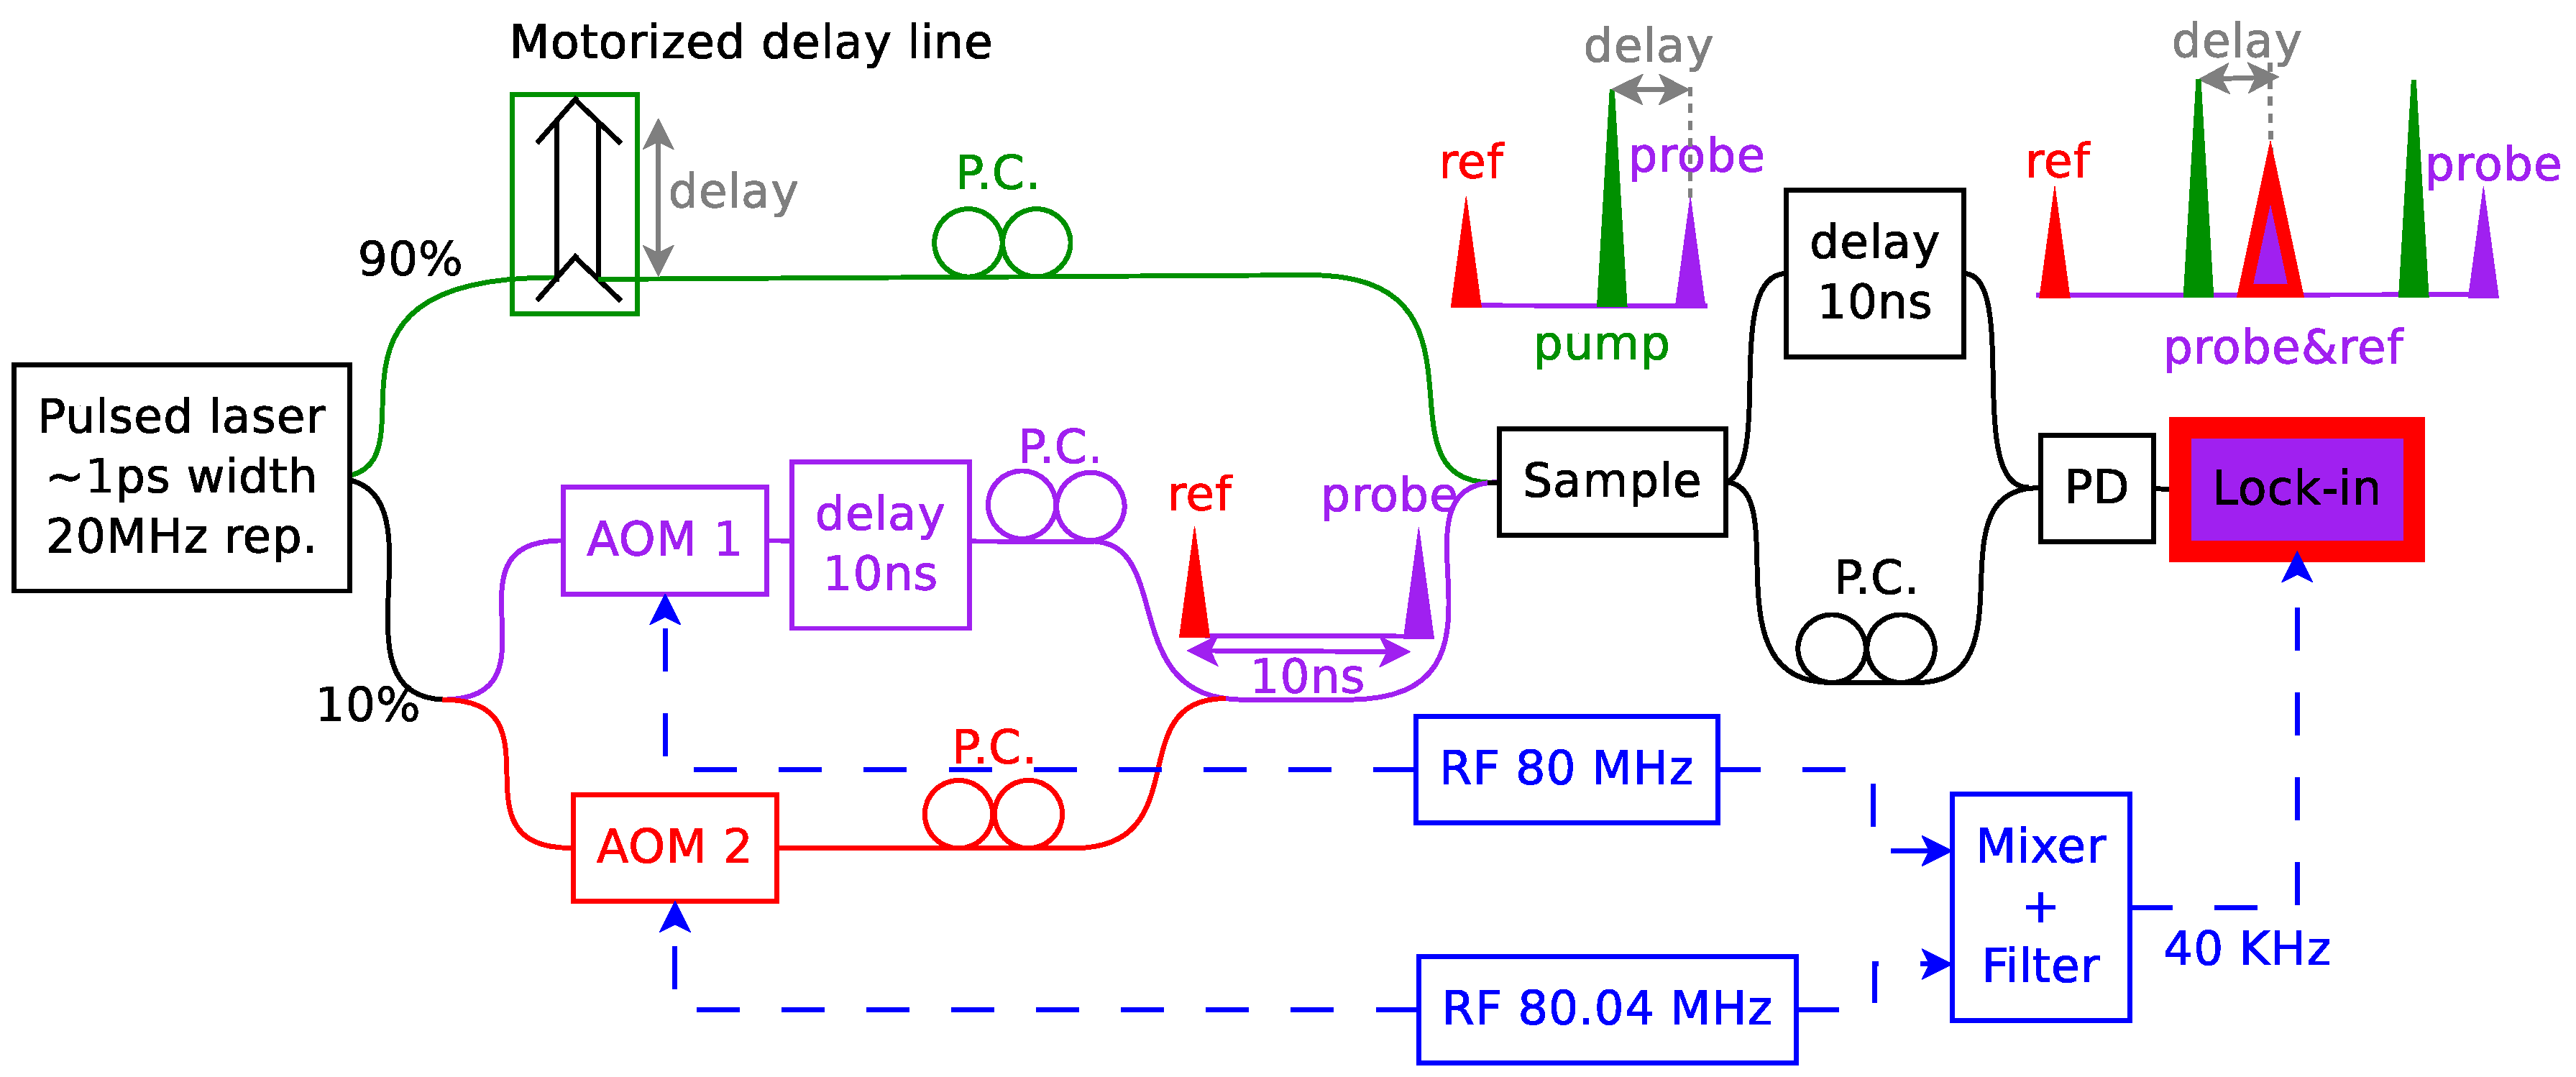
\includegraphics[width=0.95\textwidth]{timeResolved9}
                                         \caption{Time resolved characterization setup. PD: photodiode, PC: polarization controller, AOM: acousto-optic modulator.}
                                     \label{fig:setupTimeRes}
                                \end{figure}



In Fig.~\ref{fig:timeResolvesMeasurements} we observe the impact on transmission through the considered structures of both Kerr and carrier effect. The two effects produce opposite phase shifts because Kerr-effect increases the refractive index ($\Delta n > 0 $) and carriers decrease it ($ \Delta n < 0 $).  The dynamics  of these processes are also very different. During the pump pulse, an instantaneous phase change is due to Kerr effect; conversely after the pump pulse is gone, there is a phase response due to the carrier plasma effect (generally indicated as free-carrier dispersion - FCD) with positive sign that decays only on a much longer nanosecond time-scale.


\section{Time-resolved simulations}
We used the nonlinear Schr\"{o}dinger equation to simulate the propagation of pump and probe pulses in the optical waveguides~\cite{Agrawal2001a} and to fit Re$(\gamma)$. We solved the equation with the symmetrized split-step Fourier method as in~\cite{Lin2007}, by considering previously measured waveguide losses, group velocity dispersion~\cite{Mas2012} and the TPA coefficients reported in section 3 of this paper (see Table~\ref{tab:results}). The output of the simulation is the envelope of the pump, probe and reference pulses, so in order to extract the output of the lock-in amplifier we calculated the phase of the overlap-integral between the probe and reference pulses, which is equivalent to evaluate the phase of their beating signal under the assumption that the lock-in bandwidth is significantly smaller than the beating frequency:

                                                                \begin{equation}
                                                                        |T_{A}|e^{j\phi} =
                                                                        \frac{\int E_{\mathrm{ref}}(\tau) E^*_{\mathrm{probe}}(\tau) ~ \mathrm{d}\tau}
                                                                        {\int |E_{\mathrm{ref}}(\tau)|^2~\mathrm{d}\tau}
                                                                \end{equation}


    \vspace*{-15pt}                                                                                                                          
                                                                
\begin{figure}[htb]
  \centering
  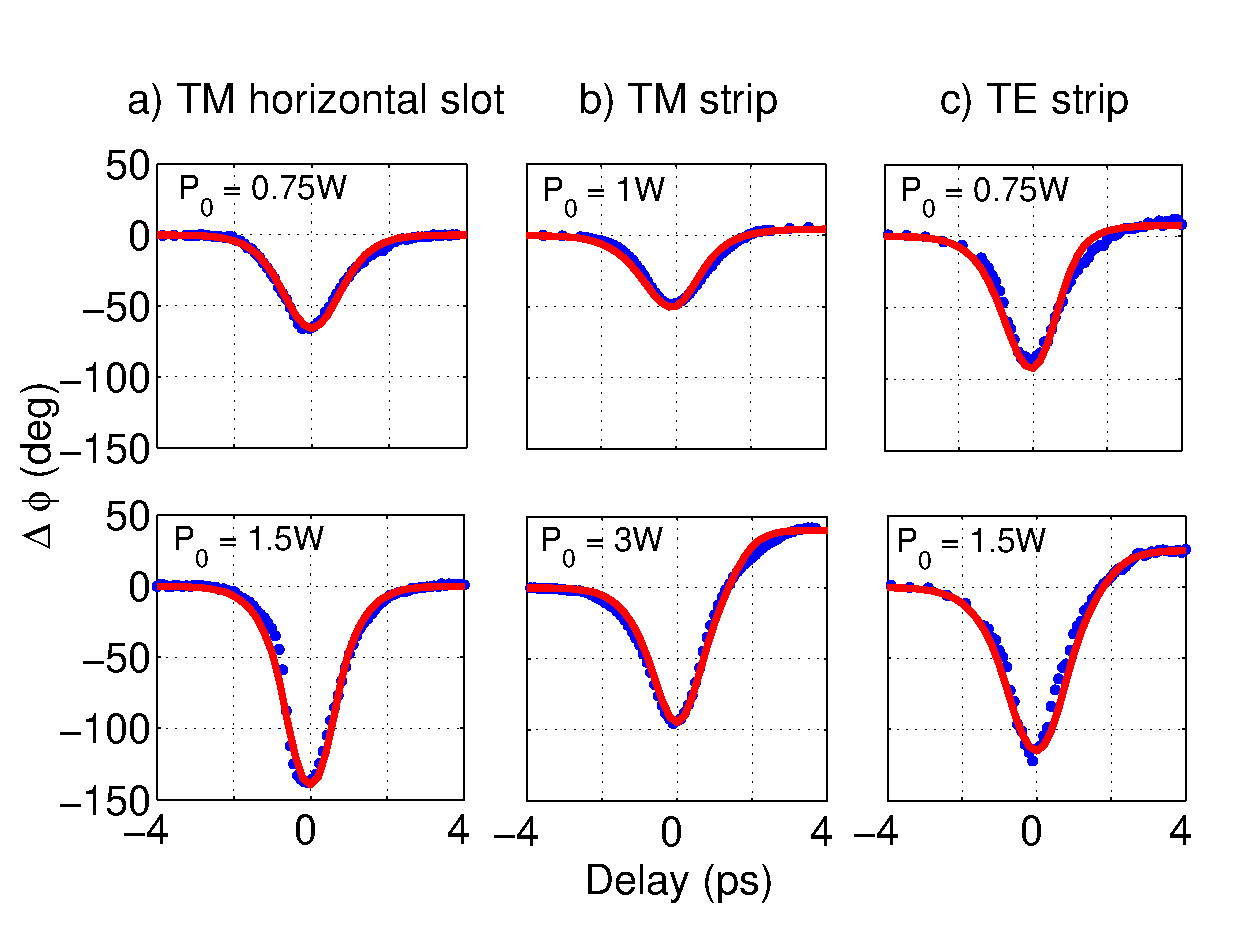
\includegraphics[width=0.77\textwidth]{measurements_v9} %COMPLETA_11
  \caption{Time resolved measurements (blue dotted curves) and simulations (red continuous curves). Samples a)TM-slot (0.75 and 1.5~W peak power) b)TM-strip (1 and 3~W peak power) c)TE-strip (0.75 and 1.5~W peak power).}
  \label{fig:timeResolvesMeasurements}
\end{figure}

where $T_A$ and $\phi$ are the amplitude and phase measured by the lock--in amplifier.
To evaluate Re$(\gamma)$ from the experimental data we performed numerical simulations (using a routine based on the split-step propagation method) in order to identify the Re$(\gamma)$ value yielding the best fit of the phase curve for each structure. In order to check for the results consistency we performed the experiments at two different power levels, obtaining two slightly different Re$(\gamma)$-values for each structure. In Table~\ref{tab:results} we report for each waveguide the average Re$(\gamma)$-value and its mean absolute deviation. 
The obtained results confirm that the slot-TM waveguide exhibits a higher nonlinear efficiency with respect to strip waveguides, that can be attributed to the high field confinement and to the interaction with silicon nanocrystals.


\section{Results and conclusion}
The first significant result is that phase measurements clearly show that the slot waveguide has not only a low TPA but also that free carriers have a negligible role. This is clear from Fig. 4 where the phase-curve is only slightly affected by the free-carrier contribution. On the contrary the response of strip waveguides shows a long tail with $\Delta n >0$ for delay times longer than 1 ps. This is confirmed by the FCD parameter, defined in~\cite{Lin2007} and shown in Table \ref{tab:results} (we have considered the effective FCD, which is normalized with the effective area, making it a device parameter like $\gamma$, rather than a material parameter). This feature considerably reduces the undesired patterning effects when modulating a real bit pattern. On the other hand, the figure of merit (FOM) given by the ratio between Kerr effect and TPA is also significantly higher in the slot waveguide than in the strip waveguides: $2.9\pm 0.06$ for the slot, $0.44 \pm 0.05$ and $0.27 \pm 0.05$ respectively for 
the TM and TE strip waveguides, as reported in Table~\ref{tab:results}. 

All these findings can be explained by the fact that in the slot waveguide, a considerable amount of energy travels through the slot layer, which provides a very efficient Kerr effect~\cite{Trita2011} and a weak TPA. Nevertheless we note that the optical performance of such waveguides depends on their structure as well as on the conditions of deposition of both the silicon nanocrystals layer and the Si top layer. On the other hand, comparing the TM and TE strips, we find that the TM has a higher FOM but lower $\gamma$ than the TE. This is expected, as the TM mode is weakly confined in the vertical direction, therefore more energy travels through the cladding, which has lower Kerr coefficient and negligible TPA.

These results agree with the ones shown in Ref.~\cite{Vallaitis2008} for a polymer-filled vertical slot; however, our system, being made of inorganic materials and only requiring CMOS processes, is expected to provide more robust and stable devices with less temperature constraints. 
In conclusion, ultrafast nonlinear measurements show that silicon-nanocrystal-based horizontal slot waveguides show weaker carrier effects and better FOM than Si strip waveguides. This makes the slot structure better suited for CMOS-compatible high-speed all-optical processing than simple Si strip waveguides.
                \begin{table}[h]
                        \centering
			\caption{Extracted linear and nonlinear parameters from the experiment for the three samples: the horizontal slot, the  485$\times$220~nm TM strip and the  445$\times$220~nm TE strip waveguide. Dispersion values obtained with the technique shown in paper \cite{Mas2012}.}
                                \begin{tabular}{l|ccc}
                                        \hline
                                        Sample & TM slot & TM strip & TE strip\\\hline
                                        Coupling loss (dB) & 8 & 6 & 6\\
                                        Propagation loss (dB/cm) & 12 & 1.9 & 4.9\\
                                        $L_{eff}$ (mm) & 3.1 & 15.2 & 8.3\\
                                        Dispersion  (ps/(km$\cdot$nm))  & -1110 & -19800 & -1200\\
                                        $ Im(\gamma)~(\mathrm{W}\cdot \mathrm{m})^{-1} $          & -11.8 & -5.4 & -68.1\\
                                        $ Re(\gamma)~(\mathrm{W}\cdot \mathrm{m})^{-1} $          & 428$\pm$ 8 & 30 $\pm$ 3 & 235 $\pm$ 30\\
                                        $ FOM = \frac{1}{4\pi} \frac{Re(\gamma)}{|Im(\gamma)|} $  & 2.9 $\pm 0.06$ & 0.44 $\pm 0.05$ & 0.27$\pm 0.05$ \\
                                        effective FCD $ \frac{-\sigma_n}{ A_{eff} }~(10^{-15}~\mathrm{m}) $  & \textless 2 & 21 & 28 \\
                                        \hline
                                \end{tabular} 

                                        
                                        \label{tab:results}

                \end{table}


\section*{Acknowledgments}
We acknowledge EU project PHOLOGIC (FP6-IST-NMP-017158), Spanish Ministry of Science and Innovation SINADEC (TEC2008-06333) and PROMETEO/2010/087 NANOFOTONICA projects, and Universidad Polit\'ecnica de Valencia for PAID 2011/1914 and J. Matres' doctoral grant.


\end{document} 
